\chapter{Eichfelder, Wechselwirkungsskalen und geladene schwache Ströme}

Quantenelektrodynamik und Quantenchromodynamik sehen im Labor sehr unterschiedlich aus, doch beide sind Eichtheorien. Tatsächlich ist nahezu jede Wechselwirkung im Standardmodell auf diese Weise organisiert. Das Wort \emph{Eich} hat eine tiefere Bedeutung, die lokale Symmetrie einschließt; auf diesen Formalismus können wir jedoch zunächst verzichten. Für den Augenblick genügt eine minimale physikalische Beschreibung: Eine Eichtheorie enthält Maxwell-artige Felder, erhaltene Quellen, Symmetrietransformationen, Eichbosonen und Regeln für die Emission und Absorption dieser Bosonen.

\section{Die Maxwell-Theorie als Prototyp}

\subsection{Felder und Potentiale}

Das elektromagnetische Feld hat sechs Komponenten: drei Komponenten des elektrischen Feldes und drei des magnetischen Feldes. Dieselbe Information lässt sich mit einer gewissen Redundanz in einem Vierer-Vektorpotenzial kodieren
\begin{equation}
A_\mu=(A_0,\boldsymbol A),
\end{equation}
wobei \(A_0\) das elektrostatische Potenzial und \(\boldsymbol A\) das räumliche Vektorpotenzial ist. Im elektrostatischen Grenzfall erhält man das elektrische Feld aus dem räumlichen Gradienten,
\begin{equation}
\boldsymbol E=-\boldsymbol\nabla A_0,
\qquad
\boldsymbol F=q\boldsymbol E,
\end{equation}
während das magnetische Feld gegeben ist durch
\begin{equation}
\boldsymbol B=\boldsymbol\nabla\times\boldsymbol A.
\end{equation}
Das Vorzeichen in der ersten Gleichung hängt von der üblichen Definition des Potenzials ab; in der Tafelbesprechung geht es vor allem darum, dass die Felder Ableitungen der Potenziale sind.
\editorialnote{Für zeitabhängige Felder lautet die vollständige Beziehung
\(\boldsymbol E=-\boldsymbol\nabla A_0-\partial_t\boldsymbol A\). Hier beschränkt sich die Vorlesung bewusst auf den einfacheren elektrostatischen Fall.}

\begin{figure}[htbp]\centering
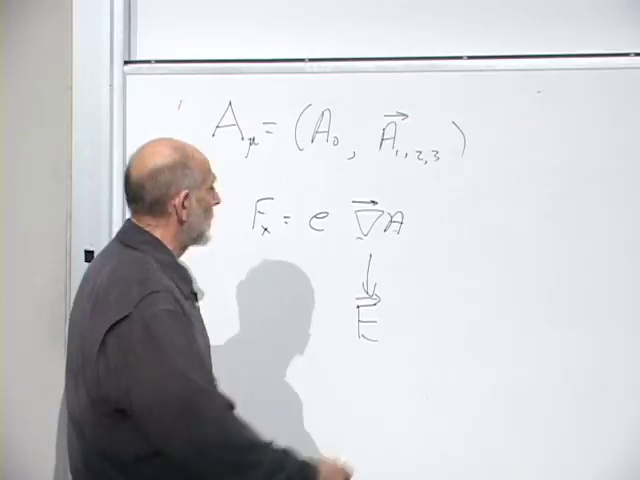
\includegraphics[width=0.62\textwidth]{lecture_05_figure_02.png}\caption{Das elektromagnetische Viererpotenzial und seine Ableitungsbeziehung zum Feld.}\lectureframe{00:03:33}\end{figure}

Damit gibt es in der Elektrodynamik zwei gleichwertige Beschreibungen: eine durch \(\boldsymbol E\) und \(\boldsymbol B\) und eine durch \(A_\mu\). Die zweite enthält nur vier angegebene Komponenten, weil verschiedene Potenziale dieselben physikalischen Felder beschreiben können. Diese Redundanz ist ein erster Hinweis auf die Bedeutung des Wortes Eichung, auch wenn wir den Begriff vorerst noch nicht formal verwenden.

\subsection{Wellen und Polarisation}

Die Maxwell-Gleichungen lassen Wellen zu. Betrachten wir eine ebene Welle, die sich entlang des Einheitsvektors \(\hat{\boldsymbol k}\) ausbreitet. An jedem Punkt stehen die elektrischen und magnetischen Felder quer zur Ausbreitungsrichtung:
\begin{equation}
\boldsymbol E\cdot\hat{\boldsymbol k}=0,
\qquad
\boldsymbol B\cdot\hat{\boldsymbol k}=0,
\qquad
\boldsymbol E\cdot\boldsymbol B=0.
\end{equation}
In Einheiten mit \(c=1\) sind ihre Beträge gleich:
\begin{equation}
|\boldsymbol E|=|\boldsymbol B|.
\end{equation}
Bei einer linear polarisierten Welle legt die Richtung von \(\boldsymbol E\) die Polarisation fest. Das gesamte Muster breitet sich mit Lichtgeschwindigkeit aus.

Die Quantisierung ändert die Beschreibung, aber nicht die Polarisationsstruktur. Ein Quant der elektromagnetischen Welle ist ein Photon. Ein Photon als Punkt darzustellen, ist zwangsläufig irreführend; dennoch kann man sich vorstellen, dass der Punkt einen kleinen, quer zur Ausbreitungsrichtung stehenden Zeiger trägt, der seine Polarisation angibt. Eine Viertelwellenplatte oder ein anderes optisches Element kann diese Polarisation drehen. Auch ein statisches Coulomb-Feld lässt sich, wenn auch nur grob, so auffassen, als entstehe es durch wiederholte Emission und Absorption von Photonen.

\subsection{Quellen, Fluss und Erhaltung}

Elektromagnetische Wellen können sich im leeren Raum ausbreiten, doch das Feld hat auch Quellen: elektrische Ladungen und Ströme. Eine positive Punktladung erzeugt ein radial nach außen gerichtetes elektrisches Feld, dessen Stärke proportional zu \(1/r^2\) ist. Die Zahl der Feldlinien, die eine beliebige Kugel um die Ladung durchstoßen, ist unabhängig vom Radius der Kugel. Mathematisch gilt in SI-Einheiten:
\begin{equation}
\oint_{S^2}\boldsymbol E\cdot d\boldsymbol S
=\frac{Q_{\mathrm{enc}}}{\epsilon_0},
\label{eq:l5-gauss}
\end{equation}

Das ist mehr als eine praktische Methode, das Feld zu berechnen. Elektrische Feldlinien können nur an Ladungen enden. Würde eine einzelne isolierte Ladung einfach verschwinden, müsste entweder ihr Feld überall gleichzeitig verschwinden, was der Kausalität widerspräche, oder eine Front des fehlenden Feldes müsste sich nach außen ausbreiten, wobei Feldlinien im leeren Raum endeten. Beides ist unzulässig. Die Geometrie des Flusses macht die Ladungserhaltung daher plausibel: Ladung kann sich bewegen, und entgegengesetzte Ladungen können annihilieren, aber die Nettoladung kann nicht lokal ohne einen kompensierenden Strom verschwinden.

Die entsprechende lokale Aussage ist die Kontinuitätsgleichung
\begin{equation}
\partial_t\rho+\boldsymbol\nabla\cdot\boldsymbol J=0.
\label{eq:l5-continuity}
\end{equation}
\editorialnote{~\eqref{eq:l5-continuity} ist die übliche lokale mathematische Form des Kausalitätsarguments über den Fluss, das in der Vorlesung verbal entwickelt wird.}

\subsection{Eine Arbeitsdefinition der Eichtheorie}

Wir können das Grundmuster nun operational formulieren. Eine Eichtheorie umfasst:
\begin{itemize}\item elektrizitätsartige und magnetismusartige Felder;
\item Wellen, die bei hinreichend schwachen Wechselwirkungen Lichtwellen ähneln;
\item Quellen, die der elektrischen Ladung entsprechen;
\item ein Gaußsches Gesetz, das den Fluss mit diesen Quellen verknüpft;
\item ein Erhaltungsgesetz und eine zugehörige Symmetrie;
\item Quanten des Feldes, sogenannte Eichbosonen; und
\item eine Kopplungskonstante, die Emission und Absorption bestimmt.
\end{itemize}
Die Quelle muss keine elektrische Ladung sein. Als bewusst unphysikalisches Beispiel stellen wir uns vor, die Baryonenzahl wäre eine Eichladung. Protonen und Neutronen haben beide die Baryonenzahl \(+1\), sodass sie sich durch eine neue, Coulomb-artige Kraft abstoßen würden; ein Proton und ein Antiproton würden sich anziehen. Eine solche Theorie ist mathematisch denkbar, doch in der Natur gibt es kein beobachtetes langreichweitiges Eichfeld, das an die Baryonenzahl koppelt. Erhaltung allein garantiert keine Eichkraft.

Die elektrische Ladung geht tatsächlich mit einer Symmetrie einher. Für ein geladenes Materiefeld gilt
\begin{equation}
\psi(x)\longmapsto e^{i\theta}\psi(x).
\label{eq:l5-u1}
\end{equation}
Phasensymmetrie und Ladungserhaltung sind zwei Seiten derselben Struktur. Später können wir \(\theta\) von der Raumzeit abhängen lassen und sehen, weshalb das Potenzial \(A_\mu\) benötigt wird. Hier genügt die globale Transformation, um die erhaltene Ladung zu identifizieren.

\section{Die QCD als nichtabelsches Beispiel}

\subsection{Tripletts, Antitripletts und die Gluonmatrix}

In der Quantenchromodynamik trägt ein Quarkfeld einen FarbindIndex \(i\in\{r,g,b\}\) und transformiert in der fundamentalen Darstellung von \(SU(3)\):
\begin{equation}
q'_i=U_{ij}q_j,
\qquad
U^\dagger U=\boldsymbol 1,
\qquad
\det U=1.
\label{eq:l5-q-transform}
\end{equation}
Dies ist eine Drehung in einem dreidimensionalen komplexen Farbraum, keine Drehung des gewöhnlichen Ortsraums. Die dreikomponentige Darstellung wird auch definierende Darstellung genannt.

Antiteilchenfelder werden durch die komplex konjugierten Variablen dargestellt. Die komplexe Konjugation von Gleichung~\eqref{eq:l5-q-transform} ergibt
\begin{equation}
q_i^{\prime *}=U_{ij}^*q_j^*.
\label{eq:l5-antiquark-transform}
\end{equation}
Quarks transformieren also gemäß \(\boldsymbol 3\), Antiquarks dagegen gemäß \(\bar{\boldsymbol 3}\).

\begin{figure}[htbp]\centering
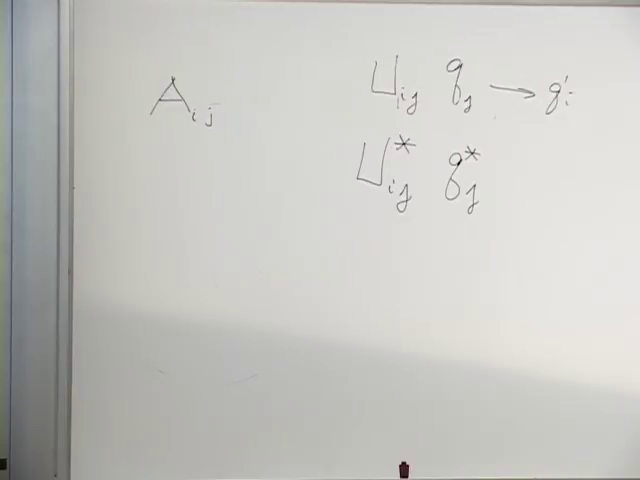
\includegraphics[width=0.62\textwidth]{lecture_05_figure_03.png}\caption{Die fundamentale Transformation und ihre komplex konjugierte Antitriplett-Transformation.}\lectureframe{00:18:47}\end{figure}

\begin{classroomqa}\audiencequestion{Wie viele \(U\)-Matrizen gibt es-- sieben, acht oder neun?
\lecturetimestamp{00:19:37}}\lecturerresponse{Es gibt unendlich viele Gruppenelemente \(U\). Gezählt wird die endliche Zahl der unabhängigen Generatoren; für \(SU(3)\) sind es acht. Eine allgemeine \(3\times3\)-Matrix hat neun Matrixeinträge, doch die spezielle Unitarität lässt acht kontinuierliche Richtungen übrig.}\end{classroomqa}

Das Gluonfeld lässt sich als spurlose Matrix \(A_{ij}\) schreiben. Ein Index transformiert wie ein Quark, der andere wie ein Antiquark; seine Farbstruktur entspricht daher
\begin{equation}
\boldsymbol 3\otimes\bar{\boldsymbol 3}
=\boldsymbol 1\oplus\boldsymbol 8.
\end{equation}
Die QCD behält das spurlose Oktett bei,
\begin{equation}
A_{ii}=\operatorname{tr}A=0,
\end{equation}
und lässt das Singulett weg. Deshalb gibt es in der QCD acht Gluonen statt neun. Allgemein hat \(SU(N)\)
\begin{equation}
N^2-1
\end{equation}
Generatoren und ebenso viele Eichbosonfelder.

Das Photon ist bezüglich der elektrischen \(U(1)\)-Symmetrie neutral: Eine Drehung der Phase eines Elektrons transformiert das Photon nicht in ein anderes Photon. Gluonen sind anders. Ein Gluon trägt eine Farbe und eine Antifarbe und transformiert daher in der adjungierten Darstellung. Eine Rot--Antiblau-Kombination ist beispielsweise kein Farbsingulett, obwohl sie eine Farbe und eine Antifarbe enthält.

\subsection{Indexfluss und Selbstwechselwirkung}

Die Wechselwirkungsregel lässt sich durch Verfolgen der Indizes ablesen. Schematisch kann ein Quark der Farbe \(i\) unter Emission eines Gluons mit entsprechendem Farbfluss zu einem Quark der Farbe \(j\) werden:
\begin{equation}
q_i\longrightarrow q_j+A_{ij}.
\label{eq:l5-quark-gluon-vertex}
\end{equation}
Die genaue Anordnung von \(i\) und \(j\) hängt von der Pfeilkonvention ab; entscheidend ist, dass jeder an einem Vertex eintretende Index über eine andere Linie weitergeführt wird. Kein Farbindex geht verloren.

Diese Regel gilt in jeder \(SU(N)\)-Eichtheorie. Fundamentale Materie hat einen Index, antifundamentale Materie einen konjugierten Index, und ein Eichboson hat je einen von beiden. Die physikalischen Bezeichnungen können sich ändern, die Indexstruktur bleibt jedoch bestehen.

Da ein Gluon selbst Farbe trägt, kann es ein weiteres Gluon emittieren. Ein \(A_{ij}\)-Gluon kann sich über einen Zwischenindex \(k\) schematisch aufspalten:
\begin{equation}
A_{ij}\longrightarrow A_{ik}+A_{kj}.
\label{eq:l5-three-gluon-index}
\end{equation}
Dies ist kein vollständiger Yang--Mills-Vertex, zeigt aber den Farbfluss. Bei Photonen in der gewöhnlichen Elektrodynamik gibt es nichts Entsprechendes. Gluonen üben daher Kräfte auf andere Gluonen aus, und die Dynamik nichtabelscher Felder ist viel komplizierter als die lineare Maxwell-Theorie.

Eine qualitative Folge ist der Einschluss. Farbfeldlinien können nicht enden, und ihre Selbstwechselwirkung bündelt sie zu einer Röhre, die ein Quark mit einem Antiquark verbindet. Die Röhre trägt eine annähernd konstante Energie pro Längeneinheit:
\begin{equation}
V(R)\simeq \sigma R.
\end{equation}
Werden die Endpunkte weiter auseinandergezogen, wird deshalb mehr Energie gespeichert, statt isolierte Farbladung freizusetzen. Das ist die anschauliche Vorstellung eines zähen Leims: Das Feld selbst verhindert, dass farbgeladene Bestandteile als freie Teilchen entkommen.

\section{Kopplungen und die Bedeutung von „stark“ oder „schwach“}

\subsection{Ladung als Emissionsamplitude}

Eine Eichtheorie benötigt weiterhin eine Kopplungskonstante. In der QED ist die Elektronenladung \(e\) der Koeffizient des Elektron--Photon-Vertices. Sie ist eine Amplitude, und Wahrscheinlichkeiten sind die Quadrate von Amplituden. Stellen wir uns ganz praktisch vor, ein schnelles Elektron werde in einer Kathodenstrahlröhre abrupt abgebremst. Die Wahrscheinlichkeit, ein Photon abzustrahlen, ist proportional zu \(e^2\); übliche Faktoren sind in der Feinstrukturkonstante enthalten:
\begin{equation}
\alpha=\frac{e^2}{4\pi\hbar c}
\simeq \frac{1}{137}.
\label{eq:l5-alpha}
\end{equation}
In natürlichen Einheiten \(\hbar=c=1\) ist die Kopplung dimensionslos. Eine Größenordnung von einem Prozent für eine elementare Emission bedeutet, dass der Elektromagnetismus im Sinne der Störungstheorie schwach ist: Die meisten abgebremsten Elektronen geben nicht jeweils einen Schauer harter Photonen ab.

\subsection{Natürliche Einheiten verknüpfen Energie, Zeit und Abstand}

Wir setzen
\begin{equation}
c=1,
\qquad
\hbar=1.
\end{equation}
Dann haben Zeit und Strecke dieselbe Einheit, während Energie die inverse Einheit hat:
\begin{equation}
E=\hbar\omega\longrightarrow E=\omega\sim\frac1t,
\qquad
x\sim t\sim\frac1E.
\end{equation}
Hohe Energien erschließen kurze Strecken und kurze Zeiten.

Zur Orientierung gilt:
\begin{equation}
1\ {\rm eV}^{-1}
=\frac{\hbar c}{1\ {\rm eV}}
\simeq 1.97\times10^{-7}\ {\rm m}.
\end{equation}
Eine atomare Länge in der Größenordnung von \(10^{-10}\ {\rm m}\) entspricht daher ungefähr dem Kehrwert eines Kiloelektronenvolts. Dies sind Umrechnungen der Größenordnung nach, keine präzisionsspektroskopischen Angaben.

\subsection{Die Hierarchie im Atom}

Für ein typisches Atom nehmen wir
\begin{equation}
R_{\rm atom}\sim10^{-10}\ {\rm m}.
\end{equation}
Licht durchquert diese Strecke in
\begin{equation}
t_{\rm transit}^{\rm atom}\sim10^{-18}\ {\rm s}.
\end{equation}
Ein Elektron bewegt sich in einem leichten Atom jedoch nur mit einem kleinen Bruchteil der Lichtgeschwindigkeit. Im Bohr-Bild gilt \(v/c\sim\alpha\), die typische Umlaufzeit ist also länger:
\begin{equation}
t_{\rm orbit}^{\rm atom}\sim10^{-16}\ {\rm s}.
\end{equation}

Ein angeregtes Atom benötigt noch länger, um Strahlung auszusenden:
\begin{equation}
t_{\rm decay}^{\rm atom}\sim10^{-9}\ {\rm s}
\end{equation}
als grobe Abschätzung auf Vorlesungsniveau. Das physikalische Bild umfasst zwei Unterdrückungen. Die elektromagnetische Kraft bewirkt nur eine mäßige Beschleunigung, und ein beschleunigtes Elektron hat zusätzlich eine kleine Emissionswahrscheinlichkeit, die durch \(\alpha\) bestimmt wird. Die kleine Feinstrukturkonstante erzeugt somit eine Hierarchie zwischen Durchquerungs-, Umlauf- und Strahlungszerfallszeiten.

\subsection{Das Fehlen einer Hierarchie im Hadron}

Ein Hadron ist ein atomähnliches gebundenes System aus Quarks und Gluonen, doch seine Skala ist viel kleiner:
\begin{equation}
R_{\rm hadron}\sim10^{-15}\ {\rm m},
\qquad
t_{\rm transit}^{\rm hadron}\sim10^{-23}\ {\rm s}.
\end{equation}
Quarks durchqueren das Hadron praktisch auf derselben Zeitskala, und auch angeregte Hadronen, die stark zerfallen, leben ungefähr
\begin{equation}
t_{\rm orbit}^{\rm hadron}
\sim t_{\rm decay}^{\rm hadron}
\sim10^{-23}\ {\rm s}.
\end{equation}
Ein angestoßenes Hadron kann schwingen und fast so schnell ein Pion aussenden, wie es die Kausalität zulässt. Es gibt keine Trennung um sieben oder neun Größenordnungen wie innerhalb eines Atoms.

\begin{classroomqa}\audiencequestion{Folgt aus der speziellen Relativitätstheorie, dass ein Hadron nicht wesentlich schneller zerfallen kann als seine Lichtdurchquerungszeit?
\lecturetimestamp{00:47:15}}\lecturerresponse{Das ist eine sinnvolle Formulierung der Abschätzung für die Größenordnung. Starke Zerfälle laufen etwa so schnell ab, wie es die Größe des Systems zulässt; es gibt weder eine kleine Kopplung noch eine andere starke Unterdrückung, die sie verlangsamt.}\end{classroomqa}

Die entsprechende starke Kopplung ist daher viel größer als \(\alpha\). Für eine beispielhafte hadronische Skala gibt die Vorlesung \begin{equation}
\alpha_{\rm QCD}\sim0.2,
\end{equation} an, also einen Wert, der viel näher bei eins liegt als \(1/137\). Darin liegt der dynamische Ursprung der älteren Bezeichnung \emph{starke Wechselwirkungen}.
\editorialnote{Die QCD-Kopplung hängt von der Energie ab; \(\alpha_s\) ist daher keine feste Zahl. Der angegebene Wert ist, wie in der Vorlesung beabsichtigt, ein beispielhafter skalenabhängiger Wert.}

\begin{classroomqa}\audiencequestion{Nennt man das Analogon der starken Wechselwirkung einfach die Konstante der starken Kraft?
\lecturetimestamp{00:48:17}}\lecturerresponse{Üblicherweise nennt man sie \(\alpha_{\rm QCD}\) oder häufiger \(\alpha_s\). Die elektromagnetische Kopplung heißt meist einfach \(\alpha\); wenn beide in derselben Diskussion vorkommen, kann man aber \(\alpha_{\rm QED}\) verwenden.}\end{classroomqa}

\begin{classroomqa}\audiencequestion{Würde man in einer wissenschaftlichen Arbeit zwischen einer nackten elektromagnetischen Kopplung und dem gemessenen, abgeschirmten Wert unterscheiden?
\lecturetimestamp{00:48:38}}\lecturerresponse{Ja. Man spricht von einer nackten Kopplung und einer renormierten Kopplung. Die Vakuumpolarisation bewirkt, dass die effektive Kopplung von der Skala abhängt, auf der sie gemessen wird.}\end{classroomqa}

\section{Das Rätsel des schwachen Zerfalls}

Die schwachen Wechselwirkungen erhielten ihren Namen wegen der sehr langen Zerfallszeiten. Zerfälle durch die schwache Wechselwirkung sind gewöhnlich langsamer als starke Zerfälle und können sogar langsamer sein als atomare Strahlungsprozesse. Das älteste Beispiel ist der nukleare Betazerfall.

\subsection{Der Betazerfall des Neutrons}

Ein freies Neutron zerfällt über
\begin{equation}
n\longrightarrow p+e^-+\bar\nu_e.
\label{eq:l5-neutron-decay-intro}
\end{equation}
Die Vorlesung setzt eine Lebensdauer von ungefähr zwölf Minuten an, absurd lang im Vergleich zu \(10^{-23}\ {\rm s}\). Für die Argumentation kommt es auf moderne Präzisionswerte nicht an.

Ein Teil der langen Lebensdauer ist kinematisch bedingt. Grob gilt:
\begin{equation}
\begin{aligned}
m_n&\simeq940\ {\rm MeV},
&
m_p&\simeq939\ {\rm MeV},
\\
m_e&\simeq0.5\ {\rm MeV}.
\end{aligned}
\end{equation}
Nur ein winziger Bruchteil der Ruheenergie des Neutrons steht als kinetische Energie zur Verfügung. Wäre das Neutron leichter als die Summe der Ruheenergien der Endteilchen, wäre der Zerfall unmöglich. Läge es nur infinitesimal oberhalb der Schwelle, wäre der verfügbare Phasenraum winzig und der Zerfall langsam. Doch der Phasenraum allein kann keine in Minuten gemessene Lebensdauer erklären.

\subsection{Das geladene Pion beseitigt den Einwand mit der Energieschwelle}

Betrachten wir auch
\begin{equation}
\pi^-\longrightarrow e^-+\bar\nu_e
\end{equation}
und den ladungskonjugierten Prozess. Das Pion hat reichlich Energie oberhalb der Elektronenschwelle, dennoch liegt seine schwache Lebensdauer in der Größenordnung von Nanosekunden und nicht bei der hadronischen Größenordnung von \(10^{-23}\) Sekunden. Ein ähnlicher Zerfallskanal mit einem Myon wird gleich wichtig. Das Rätsel ist also der schwachen Wechselwirkung selbst zuzuschreiben und nicht bloß ein Zufall der nahezu entarteten Neutronenmassen.

\editorialnote{Die Lebensdauer des geladenen Pions beträgt etwa \(26\ {\rm ns}\); der dominante Zerfallskanal ist \(\pi^-\to\mu^-\bar\nu_\mu\). Der Elektronenkanal ist helicitätsunterdrückt. In der Vorlesung wird zunächst der Elektronenkanal verwendet, weil sich dabei die Teilchen am einfachsten bilanzieren lassen; anschließend wird auf den dominanten Myonenkanal zurückgekommen.}

Die Bezeichnung Betazerfall geht historisch darauf zurück, dass emittierte Elektronen Betastrahlen genannt wurden. Bei den Beispielen mit Pion und Neutron ist dieselbe geladene Stromwechselwirkung beteiligt, obwohl sich ihre Kinematik stark unterscheidet.

\section{Eine Tabelle der Quarks und Leptonen}

\subsection{Die Farbe wirkt vertikal}

Ordnen wir die sechs Quarkflavours in drei Spaltenpaaren an,
\begin{equation}
(u,d),\qquad(c,s),\qquad(t,b),
\end{equation}
und platzieren wir eine rote, grüne und blaue Kopie jedes Quarks in getrennten Zeilen. Die Farbe \(SU(3)\) wirkt vertikal: Sie transformiert rote, grüne und blaue Varianten eines Up-Quarks ineinander und führt dieselbe Farbrotation zugleich bei Down-, Charm-, Strange-, Top- und Bottom-Quarks aus. Sie verwandelt kein Up-Quark in ein Down-Quark.

\subsection{Der schwache Isospin wirkt horizontal}

Die schwache Symmetrie wirkt in der anderen Richtung. Sie mischt jeweils die benachbarten Paare
\begin{equation}
Q_1=\begin{pmatrix}u\\d\end{pmatrix},
\qquad
Q_2=\begin{pmatrix}c\\s\end{pmatrix},
\qquad
Q_3=\begin{pmatrix}t\\b\end{pmatrix}.
\label{eq:l5-quark-doublets}
\end{equation}
Up-artige Quarks haben die Ladung \(+2/3\), Down-artige Quarks die Ladung \(-1/3\); die Ladung ändert sich also über jedes Paar hinweg um eine Einheit.
\editorialnote{An dieser Stelle sagt die Quelle kurzzeitig, ein Down-Quark habe die Ladung \(-2/3\). Die umgebende Subtraktion und alle folgenden Prozesse erfordern den Standardwert \(-1/3\), der hier verwendet wird.}

Da die Symmetrie auf Dubletts wirkt, ist \(SU(2)\) die natürliche Gruppe. Sie wirkt auf jede Farbkopie jedes Quarkdubletts, ohne die Farbe zu ändern.

Es gibt außerdem eine vierte Teilchenzeile ohne Farbe, die daher nicht mit Gluonen wechselwirkt: die Leptonen. Sie bilden drei weitere Dubletts,
\begin{equation}
L_e=\begin{pmatrix}\nu_e\\e^-\end{pmatrix},
\qquad
L_\mu=\begin{pmatrix}\nu_\mu\\\mu^-\end{pmatrix},
\qquad
L_\tau=\begin{pmatrix}\nu_\tau\\\tau^-\end{pmatrix}.
\label{eq:l5-lepton-doublets}
\end{equation}
Die Neutrinos sind elektrisch neutral; Elektron, Myon und Tau haben die Ladung \(-1\). Auch hier unterscheiden sich die beiden Mitglieder jeweils um eine Einheit elektrischer Ladung. Elektron, Myon und Tau haben dieselben Eichquantenzahlen, aber unterschiedliche Massen, genauso wie die drei Generationen Up-artiger oder Down-artiger Quarks dasselbe Ladungsmuster wiederholen.

\begin{figure}[htbp]\centering
\includegraphics[width=0.82\textwidth]{lecture_05_figure_05.png}\caption{Die Tafelübersicht: Die Farbe wirkt zwischen den roten, blauen und grünen Zeilen, während der schwache Isospin \(SU(2)\) die gepaarten Flavor-Spalten und die Leptonenzeile verbindet.}\lectureframe{01:03:35}\end{figure}

Die Leptonen als vierte Farbe zu bezeichnen, ist an dieser Stelle nur eine Analogie. Sie bilden zwar eine vierte Zeile in der Tabelle der schwachen Dubletts, doch die gewöhnliche QCD \(SU(3)\) transformiert keine Quarks in Leptonen.

\section{Konstruktion der geladenen schwachen Bosonen}

\subsection{Quantenzahlen der geladenen Bosonen}

Eichbosonen tragen die Transformationseigenschaften, die nötig sind, um von einem Mitglied eines Dubletts zum anderen überzugehen. Beginnen wir mit dem Leptonenpaar \(e^-\bar\nu_e\). Es hat die elektrische Ladung \(-1\), daher heißt das zugehörige geladene Eichboson \(W^-\):
\begin{equation}
W^-\sim e^-\bar\nu_e.
\end{equation}
Dieselben Quantenzahlen ergeben sich für ein Down-Quark und ein Anti-Up-Quark:
\begin{equation}
W^-\sim d\bar u.
\end{equation}
Das Symbol \(\sim\) bedeutet: hat dieselben relevanten Eichquantenzahlen wie. Es bedeutet nicht, dass das \(W\) buchstäblich ein gebundener Zustand dieser Teilchen ist. Das Antiteilchen hat die konjugierten Kombinationen:
\begin{equation}
W^+\sim e^+\nu_e\sim\bar d u.
\end{equation}

Zu den geladenen schwachen Vertices gehören
\begin{align}
e^-&\longrightarrow\nu_e+W^-,
&
\mu^-&\longrightarrow\nu_\mu+W^-,
\label{eq:l5-lepton-w}\\
d&\longrightarrow u+W^-,
&
s&\longrightarrow c+W^-,
\label{eq:l5-quark-w}
\end{align}
Mit entsprechenden Übergängen der dritten Generation, sofern sie kinematisch möglich sind. Das Eichboson bewirkt dynamisch dieselbe horizontale Mischung, die die Symmetrie auf dem Dublett bewirkt.

\begin{classroomqa}\audiencequestion{Die Ladungserhaltung legt für das emittierte Boson die Ladung \(-1\) fest. Doch weshalb laufen die Übergänge des Elektrons, des Down-Quarks und des Strange-Quarks alle über dasselbe Teilchen?
\lecturetimestamp{01:12:56}}\lecturerresponse{Das ist eine empirische Tatsache, die in der gemeinsamen schwachen Symmetrie zum Ausdruck kommt. Die Natur hätte widerspruchsfrei jeder Familie oder Quarks und Leptonen getrennt ein anderes \(W\)-artiges Boson zuordnen können. Stattdessen wirkt ein einziges \(SU(2)\) gleichzeitig auf alle Dubletts, und dieselben geladenen Eichbosonen vermitteln all diese Übergänge.}\end{classroomqa}

\subsection{Einen Vertex lesen und umkehren}

Ein einzelner Vertex steht für eine ganze Familie von Prozessen. Wird eine eintretende Linie in eine austretende umgekehrt, verwandelt sich ein Teilchen in sein Antiteilchen; wird eine \(W^-\)-Linie umgekehrt, erhält man ein \(W^+\). Ein Vertex kann daher als Emission, Absorption, Zerfall, Annihilation oder umgekehrte Reaktion gelesen werden, sofern Ladung, Impuls und alle relevanten Quantenzahlen durchgehend konsistent berücksichtigt werden.

\begin{classroomqa}\audiencequestion{Kann man die Pfeile und Linien in diesen schwachen Vertices umkehren?
\lecturetimestamp{01:14:51}}\lecturerresponse{Ja. Eine Linie kann von einem Endzustand in den Anfangszustand überführt werden oder umgekehrt; dabei wird ein Teilchen jedoch zu seinem Antiteilchen. Derselbe lokale Vertex beschreibt folglich viele unterschiedlich orientierte Reaktionen.}\end{classroomqa}

\begin{classroomqa}\audiencequestion{Bedeutet die Darstellung eines \(W^-\) mit Strange- und Charm-Linien, dass das Boson buchstäblich aus einem Strange-Quark und einem Anti-Charm-Quark besteht?
\lecturetimestamp{01:15:43}}\lecturerresponse{Nein. Die Linienbuchführung besagt lediglich, dass das \(W^-\) die Änderung der Quantenzahlen zwischen diesen Spalten vermittelt. Liest man das Diagramm als Zerfall, kann ein hinreichend energiereiches \(W^-\) ein Strange-Quark und ein Anti-Charm-Quark erzeugen; aus ihnen besteht es nicht.}\end{classroomqa}

\begin{classroomqa}\audiencequestion{Können ein Elektron und ein Antineutrino ein \(W\) bilden, das anschließend ein Quarkpaar erzeugt?
\lecturetimestamp{01:17:22}}\lecturerresponse{Genau. Ist genügend Schwerpunktsenergie verfügbar, können die einlaufenden Leptonen den Zwischenzustand des geladenen Stroms bilden, der dann über einen erlaubten Quarkkanal austreten kann. Es sind dieselben beiden Vertices wie beim Zerfall, nur anders orientiert gelesen.}\end{classroomqa}

\subsection{Das fehlende dritte Boson}

Eine \(SU(2)\)-Gruppe hat drei Generatoren und somit drei Eichfelder. Bisher haben wir nur \(W^+\) und \(W^-\) dargestellt. Mit einem dritten, elektrisch neutralen Feld müssen diagonale Kombinationen wie Elektron--Positron und Neutrino--Antineutrino-Quantenzahlen verbunden sein. Es bleibt hier bewusst im Hintergrund. Seine Beziehung zum physikalischen \(Z\)-Boson und zum Photon erfordert eine elektroschwache Mischung, die später behandelt wird.

\begin{classroomqa}\audiencequestion{Wurden die schwache und die starke Kraft zu unterschiedlichen Zeiten vermutet?
\lecturetimestamp{01:24:11}}\lecturerresponse{Ihre experimentellen Ursprünge traten gemeinsam bei der frühen Erforschung der Radioaktivität zutage. Der Alphazerfall gab Aufschluss über Kernphysik und starke Wechselwirkungen, der Betazerfall über die schwache Wechselwirkung, und beim Gammazerfall wurden elektromagnetische Photonen emittiert. Schon in der Zeit Becquerels gab es alle drei Hinweise, lange bevor die modernen Feldtheorien dazu entwickelt wurden.}\end{classroomqa}

\section{Beispiele für Zerfälle über geladene Ströme}

\subsection{Der Pionzerfall}

Das negativ geladene Pion hat den Valenzquarkinhalt
\begin{equation}
\pi^-=d\bar u.
\end{equation}
Diese Quantenzahlen können zu einem \(W^-\) annihilieren, das anschließend ein geladenes Lepton und das zugehörige Antineutrino erzeugen kann:
\begin{align}
\pi^-&\longrightarrow W^{-*}
\longrightarrow e^-+\bar\nu_e,
\label{eq:l5-pion-electron}\\
\pi^-&\longrightarrow W^{-*}
\longrightarrow \mu^-+\bar\nu_\mu.
\label{eq:l5-pion-muon}
\end{align}
Der Stern erinnert daran, dass das Zwischen-\(W\) virtuell ist. Der zweite Kanal ist der dominante.

\begin{figure}[htbp]\centering
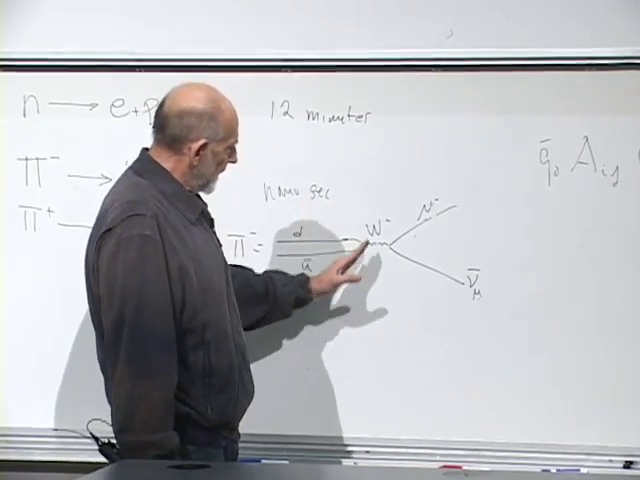
\includegraphics[width=0.72\textwidth]{lecture_05_figure_04.png}\caption{Ein \(d\bar u\)-Pion annihiliert zu einem virtuellen \(W^-\); anschließend entstehen ein geladenes Lepton und das zugehörige Antineutrino.}\lectureframe{01:19:38}\end{figure}

\begin{classroomqa}\audiencequestion{Ist dies wirklich ein Feynman-Diagramm, obwohl die Zeitrichtung horizontal statt vertikal eingezeichnet ist?
\lecturetimestamp{01:20:21}}\lecturerresponse{Ja. Die Orientierung der Zeit auf der Seite ist Konvention. Sobald eine Richtung als Zeit festgelegt und alle Pfeile konsistent interpretiert werden, enthält die Zeichnung dieselbe Information über die Wechselwirkung.}\end{classroomqa}

\begin{classroomqa}\audiencequestion{Kann man das Diagramm eher als umkehrbare chemische Reaktion denn als unumkehrbaren Zerfall lesen?
\lecturetimestamp{01:21:35}}\lecturerresponse{Der umgekehrte Prozess ist erlaubt. Ein im leeren Raum erzeugtes Pion zerfällt, weil sich die austretenden Teilchen voneinander entfernen und gewöhnlich nicht wieder zusammenkommen. Werden jedoch ein Myon und ein Antineutrino mit der passenden Energie und dem passenden Impuls gemeinsam aufeinander geschossen, gibt es eine von null verschiedene Amplitude dafür, dass sie über die umgekehrte Wechselwirkung ein Pion bilden.}\end{classroomqa}

\subsection{Energie und ein virtueller Zwischenzustand}

Für ein ruhendes Pion gilt
\begin{equation}
m_\pi\simeq140\ {\rm MeV},
\qquad
m_\mu\simeq106\ {\rm MeV},
\qquad
m_\nu\approx0
\end{equation}
mit der hier relevanten Genauigkeit. Die verbleibende Energie wird zur kinetischen Energie der austretenden Teilchen. Aus der Impulserhaltung folgt
\begin{equation}
\boldsymbol p_\mu+\boldsymbol p_{\bar\nu}=0,
\end{equation}
Die beiden Teilchen verlassen das Pion-Ruhesystem also in entgegengesetzte Richtungen.

\begin{classroomqa}\audiencequestion{Wie kann die Energie erhalten bleiben, wenn das Zwischen-\(W\) viel schwerer ist als das Pion?
\lecturetimestamp{01:25:08}}\lecturerresponse{Nur die Anfangs- und Endteilchen müssen auf ihrer Massenschale liegen. Der Viererimpuls ist an jedem Vertex erhalten, aber eine interne virtuelle Linie muss \(E^2=\boldsymbol p^2+m_W^2\) nicht erfüllen. Je größer ihre Abweichung von der Massenschale ist, desto stärker unterdrückt ihr Propagator den Prozess.\editorialnote{Die Vorlesung verwendet die traditionelle Sprache der Energie--Zeit-Unschärfe und sagt, der Zwischenzustand könne kurzzeitig die Energie verletzen. Die präzise moderne Aussage ist die in der Antwort: Energie und Impuls sind erhalten, während eine virtuelle interne Linie nicht die Massenschalenbedingung für reale Teilchen erfüllen muss.}}\end{classroomqa}

\subsection{Der Myonzerfall}

Ein Myon kann sich zunächst durch Emission eines virtuellen \(W^-\) in sein eigenes Neutrino umwandeln:
\begin{equation}
\mu^-\longrightarrow\nu_\mu+W^{-*}.
\end{equation}
Das virtuelle Boson erzeugt dann ein Elektron und ein Elektron-Antineutrino:
\begin{equation}
\mu^-\longrightarrow
\nu_\mu+e^-+\bar\nu_e.
\label{eq:l5-muon-decay}
\end{equation}
Dies ist ein rein leptonischer Prozess. Das Myon ist etwa zweihundertmal schwerer als das Elektron, sodass die Ruheenergien der Endteilchen reichlich kinetische Energie übrig lassen.

\begin{figure}[htbp]\centering
\includegraphics[width=0.72\textwidth]{lecture_05_figure_06.png}\caption{Myonzerfall über ein virtuelles geladenes schwaches Boson.}\lectureframe{01:29:24}\end{figure}

\begin{classroomqa}
\audiencequestion{Ist das neutrale Teilchen, das zusammen mit dem Elektron emittiert wird, ein Antineutrino?
\lecturetimestamp{01:29:06}}
\lecturerresponse{Ja. Der vollständige Endzustand enthält ein Myon-Neutrino, ein Elektron-Antineutrino und das Elektron. Anhand der Flavour-Bezeichnungen lassen sich die beiden neutralen Teilchen auseinanderhalten.
}
\end{classroomqa}

Das Elektron kann diesen Zerfall im leeren Raum nicht umkehren, weil es leichter als das Myon ist. Das Tau ist schwerer und kann über analoge schwache Kanäle zerfallen. Die Stabilität ist hier teilweise ein Zufall der Massenordnung und kein Unterschied im zugrunde liegenden Vertex.

\begin{classroomqa}
\audiencequestion{Erhöht ein Linearbeschleuniger effektiv die Masse des Elektrons, sodass andernfalls verbotene Reaktionen in umgekehrter Richtung ablaufen können?
\lecturetimestamp{01:30:23}}
\lecturerresponse{Er ändert nicht die invariante Ruhemasse des Elektrons, sondern stellt kinetische Energie bereit. Eine ausreichend hohe Schwerpunktsenergie kann schwerere Endzustandsteilchen erzeugen. Die zugrunde liegende physikalische Vorstellung stimmt also, wenn man Masse durch die verfügbare Kollisionsenergie ersetzt.
}
\end{classroomqa}

\subsection{Neutronen-Betazerfall auf Quarkebene}

Die Valenzquarkzusammensetzungen von Neutron und Proton sind
\begin{equation}
n=udd,
\qquad
p=uud.
\end{equation}
Ein Down-Quark im Neutron geht über den geladenen Strom in den Übergang
\begin{equation}
d\longrightarrow u+W^{-*},
\end{equation}
wobei \(udd\) in \(uud\) übergeht. Das virtuelle Boson zerfällt anschließend:
\begin{equation}
W^{-*}\longrightarrow e^-+\bar\nu_e.
\end{equation}
Zusammen ergeben die beiden Vertizes
\begin{equation}
n\longrightarrow p+e^-+\bar\nu_e.
\end{equation}

Der umgekehrte Quarkübergang \(u\to d+W^+\) würde ein Baryon aus drei Down-Quarks ergeben. Dieser mögliche Zustand ist jedoch zu schwer, als dass ein freies Neutron ihn erzeugen könnte. Der tatsächliche Übergang von Down zu Up ist energetisch erlaubt.

\begin{classroomqa}
\audiencequestion{Könnte ein Neutron stattdessen in ein Proton, ein Myon und das entsprechende Antineutrino zerfallen?
\lecturetimestamp{01:32:38}}
\lecturerresponse{Nicht bei einem freien Neutron in Ruhe: Die Massendifferenz zwischen Neutron--und Proton ist viel kleiner als die Myonmasse. Mit genügend zusätzlicher Kollisions- oder Anregungsenergie kann derselbe schwache Vertex an einem Kanal beteiligt sein, in dem ein Myon entsteht. Das Verbot ist kinematischer Art und beruht nicht auf einer fehlenden Wechselwirkung.
}
\end{classroomqa}

\section{Die ungeklärte Unterdrückung}

Die geladenen schwachen Vertizes erklären, welche Prozesse stattfinden können, aber noch nicht, warum sie so langsam ablaufen. Eine verlockende Erklärung wäre eine außerordentlich kleine schwache Kopplung. Das ist jedoch falsch: Die dimensionslose schwache Eichkopplung ist ungefähr so groß wie die elektromagnetische. Die Unterdrückung muss also eine andere Ursache haben.

Der fehlende Baustein ist bereits im virtuellen Propagator zu erkennen: Das Boson \(W\) ist sehr massereich. Bei Energien weit unterhalb von \(m_W\) werden die Amplituden geladener Ströme ungefähr durch Potenzen von \(1/m_W^2\) unterdrückt. Dieser Zusammenhang wird später behandelt, nachdem der Higgs-Mechanismus und die elektroschwache Symmetriebrechung erklärt haben, wie die Eichbosonen Masse erhalten.
\editorialnote{Die Vorlesung lässt dieses Rätsel als Frage für die nächste Sitzung offen. Die Erklärung über das schwere \(W\)-Boson ist hier als Ausblick aufgenommen und nicht als Behauptung, dass seine Herleitung in dieser Vorlesung erfolgt sei.}

\begin{classroomqa}
\audiencequestion{Wenn wir sagen, dass die Theorie diese Symmetrie besitzt, meinen wir damit, dass ihre Lagrangefunktion unter den entsprechenden Operationen invariant ist?
\lecturetimestamp{01:34:14}}
\lecturerresponse{Genau. Die Aussage, dass die Theorie die Symmetrie besitzt, ist eine Kurzform dafür, dass die Lagrangefunktion oder gleichwertig die Wirkung unter diesen Transformationen invariant ist. Die vollständige Lagrangefunktion wird auf später verschoben, nicht durch eine andere Definition ersetzt.
}
\end{classroomqa}

Damit ist der Weg vollständig: Die Maxwell-Theorie liefert das Vorbild; die QCD zeigt, wie nichtabelsche Eichbosonen Ladung tragen und austauschen; die Kopplungskonstanten erklären den Unterschied zwischen atomaren und hadronischen Zeitskalen; und die schwache \(SU(2)\)-Symmetrie ordnet Quarks und Leptonen Dubletts zu, die durch \(W^\pm\) miteinander verbunden sind. Es bleibt zu verstehen, warum diese eichvermittelten Prozesse in der Praxis schwach sind, obwohl ihre zugrunde liegende Kopplung nicht außergewöhnlich klein ist.
